Consider the Figure \ref{fig:introPhoto}. The fish in the center and the person on the left have a high memorability score (memorability $= 0.64$) and many humans tend to remember them even after $30$ minute duration. However, humans remember the left person far more than that the person on the right (memorability $= 0.18$) even though they are both comparable in size. Interestingly, the boat is also remembered far less by humans (memorability $= 0.18$) despite covering a large portion of the image . This suggests a significant and interesting bias in perceived object memorability by human viewers!

Human long-term memory can store a remarkable amount of visual information and remember thousands of different pictures even after seeing each of them only once [25, 1]. However, it appears to be the fate of visual memories that they degrade [13, 30]. While most of the work in visual cognition has examined how people forget for general classes of visual or verbal stimuli [30], little work has looked at which image information is forgotten and which is retained. Does all visual information fade alike? Are there some features, image regions or objects that are forgotten more easily than others? Inspired by work in visual cognition showing that humans selectively forget some objects and regions from an image while retaining others [22], we propose a novel probabilistic framework for modeling image memorability, based on the fading of local image information.

\begin{figure}[t]
\centering
\subfigure{
\includegraphics[width=0.48\textwidth]{figures/introduction/113.jpg}}
\subfigure{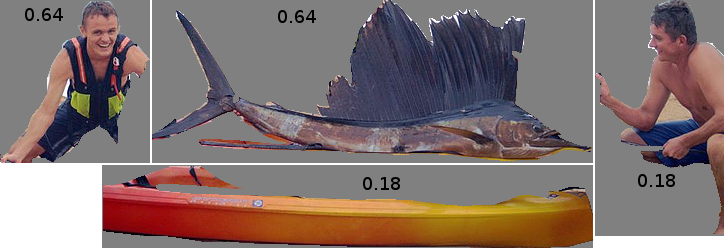
\includegraphics[width=0.48\textwidth]{figures/introduction/allObs.png}}
\vspace{-3mm}\caption{\footnotesize\textbf{Object memorability.}}\label{fig:introPhoto}
\end{figure}

Recent work on image memorability [6, 7, 12] has shown that there are large differences between the memorabilities of different images, and these differences are consistent across context and observers, suggesting that memory differences are intrinsic to the images themselves. Using machine learning tools such as support vector regression and a fully annotated dataset of images with human memorability scores, Isola et al [7] show that an automatic image ranking algorithm matches individual image memory scores quite well: with dynamic scenes with people interacting as most memorable, static indoor environments and human-scale objects as somewhat less memorable, and outdoor vistas as forgettable. In addition, using manual annotation, Isola et al. quantified the contribution of segmented regions to the image memorability score, creating a memorability map for each individual image that identifies objects that are correlated with high or low memorability scores. However, this previous work did not attempt to discover in an automatic fashion which part of the
image is memorable and which regions are forgettable.

In this paper, we introduce a novel framework for predicting image memorability that is able to
account for how memorability of image regions and different types of features fade over time, offering memorability maps that are more interpretable than [7]. The current work offers three original contributions: (1) a probabilistic model that simulates the forgetting local image regions, (2) the automatic discovery of memorability maps of individual images that reveal which regions are memorable/ forgettable, and (3) an improved overall image memorability prediction from [7], using an automatic, data-driven approach combining local and global images features. 